%%%%%%%%%%%%%%
% Reproducible research workflow + link commands (Short Example)
% Christopher Gandrud
% Updated 18 February 2013
%%%%%%%%%%%%%%

% Define colors for figure
%% Color palette (GnBU) chosen using ColorBrewer 2.0
%% See: http://colorbrewer2.org/
%% Not used in the print version
\definecolor{Blue}{HTML}{7BCCC4}
\definecolor{LiteBlue}{HTML}{A8DDB5}
\definecolor{DarkBlue}{HTML}{08589E}

\definecolor{GrayLine}{HTML}{BDBDBD}

% Set node styles
%% File nodes
\tikzstyle{File} = [draw=Blue, 
                    rectangle, 
                    text width=6.3em, 
                    font=\scriptsize]

% Raw Data nodes
\tikzstyle{RawData} = [draw=LiteBlue, 
                       %fill=LiteBlue, 
                       decorate,
                       decoration={random steps,
                                   segment length=2pt,
                                   amplitude=2pt},
                       inner sep=0.25cm, 
                       font=\scriptsize]
                    
% Separator line style
\tikzstyle{sepline} = [draw,
                        very thick,
                        color=GrayLine]
                        
% Link command nodes       
\tikzstyle{Links} = [draw=none, 
                          text width=6em,
                          text=DarkBlue,
                          font=\small]

% Begin tikz picture
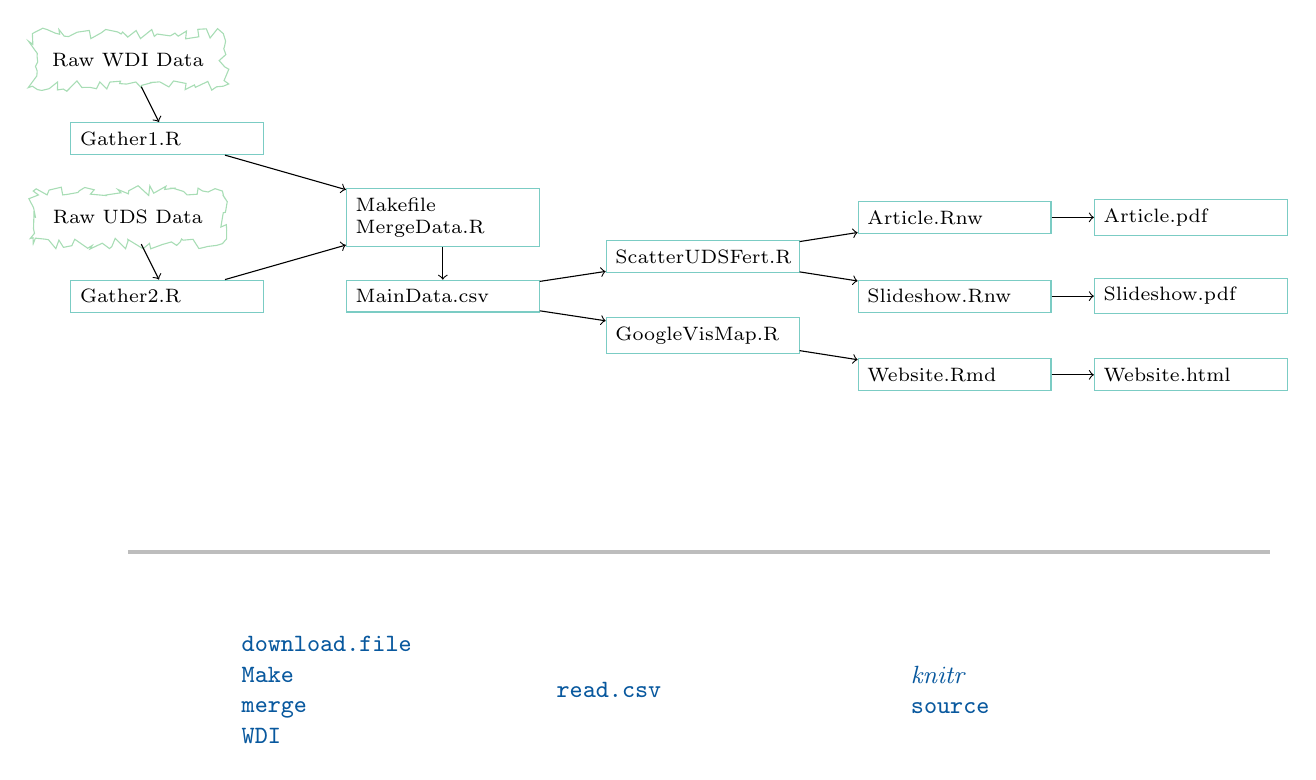
\begin{tikzpicture}

    % Nodes
    \node (Data1) at (-3.5, 7) [RawData]{Raw WDI Data};
    \node (Gather1) at (-3, 6) [File]{Gather1.R};

    \node (Data2) at (-3.5, 5) [RawData]{Raw UDS Data};
    \node (Gather2) at (-3, 4) [File]{Gather2.R};

    \node (MergeData) at (0.5, 5) [File]{Makefile \\ MergeData.R};
    \node (DataFile) at (0.5, 4) [File]{MainData.csv}; 

    \node (Scatter) at (3.8, 4.5) [File]{ScatterUDSFert.R};
    \node (GoogleVis) at (3.8, 3.5) [File]{GoogleVisMap.R};

    \node (ArticleK) at (7, 5) [File]{Article.Rnw};
    \node (SlideshowK) at (7, 4) [File]{Slideshow.Rnw};
    \node (WebsiteK) at (7, 3) [File]{Website.Rmd};

    \node (Article) at (10, 5) [File]{Article.pdf};
    \node (Slideshow) at (10, 4) [File]{Slideshow.pdf};
    \node (Website) at (10, 3) [File]{Website.html};

    % Lines
    \draw [->] (Data1) -- (Gather1);
    \draw [->] (Data2) -- (Gather2);
    \draw [->] (Gather1) -- (MergeData);
    \draw [->] (Gather2) -- (MergeData);
    \draw [->] (MergeData) -- (DataFile); 

    \draw [->] (DataFile) -- (Scatter); 
    \draw [->] (DataFile) -- (GoogleVis);  
   
    \draw [->] (Scatter) -- (ArticleK);
    \draw [->] (Scatter) -- (SlideshowK);
    \draw [->] (GoogleVis) -- (WebsiteK);

    \draw [->] (ArticleK) -- (Article);
    \draw [->] (SlideshowK) -- (Slideshow);
    \draw [->] (WebsiteK) -- (Website);
    
    
    \path [sepline] (-3.5, 0.75) -- (11, 0.75);
    
    % Link command nodes

    \node (importData) at (-1, -1) [Links]{\texttt{download.file} \\ \texttt{Make} \\ \texttt{merge}\\ \texttt{WDI} };

    \node (Figs) at (3, -1) [Links]{\texttt{read.csv}};
 
    \node (knitr) at (7.5, -1) [Links]{ {\emph{knitr}} \\ \texttt{source}};

  

  
\end{tikzpicture}